\section{Auswertung}
\label{sec:Auswertung}
\subsection{Vorbereitung}
Für die Vorbereitung soll das Dispersionsgebiet und das Auflösungsvermögen für die beiden 
verwendeten Wellenlängen bestimmt werden. Diese Größen können mit den Gleichungen \eqref{eq:del_Lam} und \eqref{eq:del_A} berechnet werden.
Die Ergebnisse sind in Tabelle \ref{tab:Vorbereitung} aufgelistet.
\FloatBarrier
\begin{table}
    \centering
    \caption{Dispersionsgebiet und Auflösungsvermögen für die beiden Wellenlängen.}
    \label{tab:Vorbereitung}
    \begin{tabular}{c c c}
        \toprule
        Wellenlänge $\lambda$ / $\SI{}{\nano\meter}$&Auflösungsvermögen $A$& Dispersionsgebiet $\Delta \lambda_{\text{D}}$ / $\SI{}{\pico\meter}$\\
        \midrule
        rot $\num{643.8}$&$\num{2.09e5}$&$\num{48.9}$\\
        blau $\num{480.0}$&$\num{2.85e5}$&$\num{27.0}$\\
        \bottomrule
    \end{tabular}
\end{table}
\FloatBarrier
Die Quantenzahlen und die mit Gleichung \eqref{len5} berechneten Landéfaktoren sind in Tabelle \ref{tab:Quantenzahlen} 
aufgelistet.
\FloatBarrier
\begin{table}
    \centering
    \caption{Quantenzahlen und Landé-Faktoren der einzelnen Zustände.}
    \label{tab:Quantenzahlen}
    \begin{tabular}{c c c c c}
        \toprule
        Zustand&S&L&J&$g_{\text{j}}$\\
        \midrule
        $^1\text{P}_1$&0&1&1&1\\
        $^1\text{D}_1$&0&2&2&1\\
        $^3\text{S}_1$&1&0&1&2\\
        $^3\text{P}_1$&1&L&1&$\num{1.5}$\\
        \bottomrule
    \end{tabular}
\end{table}
\FloatBarrier
Die Landé-Faktoren $g_{\text{ij}}$ der Übergänge werden mit der Gleichung \eqref{eq:Landeübergang} bestimmt.
\begin{equation}
    \label{eq:Landeübergang}
    g_{\text{ij}} = m_{\text{i}}g_{\text{i}} - m_{\text{j}}g_{\text{j}}
\end{equation}
Der Übergang des roten Lichtes ist $^1\text{P}_1 \rightarrow ^1\text{D}_1$ und für das 
blau Licht ist der Übergang $^3\text{S}_1 \rightarrow ^3\text{P}_1$.
Die Landé-Faktoren $g_{\text{ij}}$ der Übergänge des roten Lichtes sind in Tabelle \ref{tab:rotÜber} und die
für das blaue Licht in Tabelle \ref{tab:blauÜber} aufgelistet.
\FloatBarrier
\begin{table}
    \centering
    \caption{Landé-Faktoren der Zustände und Übergänge des roten Lichtes.}
    \label{tab:rotÜber}
    \begin{tabular}{c| c c| c c| c c}
        \toprule
        Übergang&\multicolumn{2}{c|}{Zustand i}&\multicolumn{2}{c|}{Zustand i}&\\
                &\multicolumn{2}{c|}{$^1\text{P}_1$}&\multicolumn{2}{c|}{$^1\text{D}_1$}&\\
        \midrule
        &$m_\text{i}$&$g_\text{i}$&$m_\text{j}$&$g_\text{j}$&$\Delta m $&$g_{\text{ij}}$\\
        \midrule
        \multirow{3}{*}{$\pi$}&1&\multirow{3}{*}{1}&1&\multirow{3}{*}{1}&\multirow{3}{*}{0}&\multirow{3}{*}{0}\\
        &0&&0&&&\\
        &-1&&-1&&&\\
        \hline
        \multirow{3}{*}{$\sigma^-$}&2&\multirow{3}{*}{1}&1&\multirow{3}{*}{1}&\multirow{3}{*}{-1}&\multirow{3}{*}{1}\\
        &1&&0&&&\\
        &0&&-1&&&\\
        \hline
        \multirow{3}{*}{$\sigma^+$}&0&\multirow{3}{*}{1}&1&\multirow{3}{*}{1}&\multirow{3}{*}{1}&\multirow{3}{*}{-1}\\
        &-1&&0&&&\\
        &-2&&-1&&&\\
        \bottomrule
    \end{tabular}
\end{table}
\begin{table}
    \centering
    \caption{Landé-Faktoren der Zustände und Übergänge des blauen Lichtes.}
    \label{tab:blauÜber}
    \begin{tabular}{c| c c| c c| c c}
        \toprule
        Übergang&\multicolumn{2}{c|}{Zustand i}&\multicolumn{2}{c|}{Zustand i}&\\
                &\multicolumn{2}{c|}{$^3\text{S}_1$}&\multicolumn{2}{c|}{$^3\text{P}_1$}&\\
        \midrule
        &$m_\text{i}$&$g_\text{i}$&$m_\text{j}$&$g_\text{j}$&$\Delta m $&$g_{\text{ij}}$\\
        \midrule
        \multirow{3}{*}{$\pi$}&1&\multirow{3}{*}{$\num{1.5}$}&1&\multirow{3}{*}{2}&\multirow{3}{*}{0}&$\num{-0.5}$\\
        &0&&0&&&0\\
        &-1&&-1&&&$\num{0.5}$\\
        \hline
        \multirow{2}{*}{$\sigma^-$}&1&\multirow{2}{*}{$\num{1.5}$}&0&\multirow{2}{*}{2}&\multirow{2}{*}{-1}&$\num{1.5}$\\
        &0&&-1&&&2\\
        \hline
        \multirow{2}{*}{$\sigma^+$}&0&\multirow{2}{*}{$\num{1.5}$}&1&\multirow{2}{*}{2}&\multirow{2}{*}{1}&-2\\
        &-1&&0&&&$\num{-1.5}$\\
        \bottomrule
    \end{tabular}
\end{table}
\subsection{Bestimmung des Magnetfeldes}
Um die Magnetfeldstärke bestimmen zu können, wird diese in Abhängigkeit der Stromstärke gemessen. Die Messdaten
sind in Tabelle \ref{tab:Magnetfeldstärke} aufgelistet.
\begin{table}
    \centering
    \caption{Magnetfeldstärke und Stromstärke für die Bestimmung einer Ausgleichsgeraden.}
    \label{tab:Magnetfeldstärke}
    \begin{tabular}{c c}
        \toprule
        I / $\SI{}{\ampere}$&B / $\SI{}{\milli\tesla}$\\
        \midrule
        $\num{0.45}$&$\num{39.4}$\\
        $\num{1.02}$&$\num{83.7}$\\
        $\num{1.50}$&$\num{125.7}$\\
        $\num{2.00}$&$\num{167.7}$\\
        $\num{2.50}$&$\num{209.7}$\\
        $\num{3.00}$&$\num{246.0}$\\
        $\num{3.50}$&$\num{285.4}$\\
        $\num{4.04}$&$\num{321.6}$\\
        $\num{4.49}$&$\num{352.8}$\\
        $\num{5.02}$&$\num{380.3}$\\
        \bottomrule
    \end{tabular}
\end{table}
Durch die Daten aus Tabelle \ref{tab:Magnetfeldstärke} wird eine Ausgleichsgerade der Form
\begin{equation*}
    \text{B}(\text{I}) = m\text{I} +b
\end{equation*}
gelegt.
Die Fitparameter sind 
\begin{equation*}
    m = \SI{76(1)}{\milli\tesla\per\ampere} \quad b = \SI{12(5)}{\milli\tesla}.
\end{equation*}
Die Messdaten und die Ausgleichsgerade sind in Abbildung \ref{fig:Magnetfeldstärke} abgebildet.
\begin{figure}
    \centering
    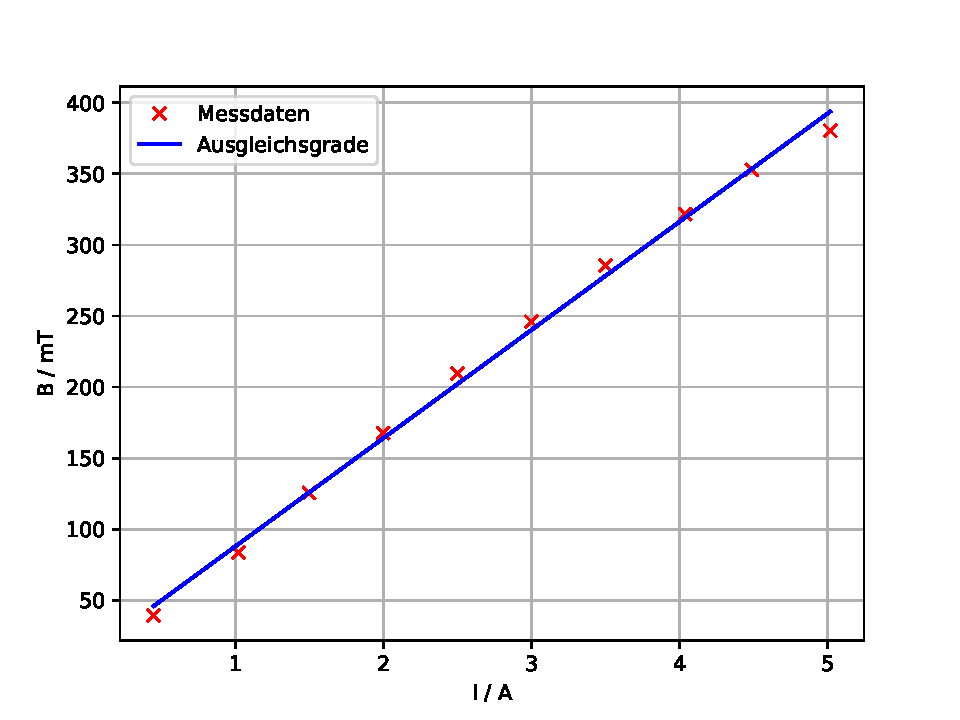
\includegraphics[width=\textwidth,keepaspectratio]{figure/B_plot.pdf}
    \caption{Messdaten und Ausgleichsgerade für die Bestimmung der Magnetfeldstärke in Abhängigkeit der Stromstärke.}
    \label{fig:Magnetfeldstärke}
\end{figure}
\FloatBarrier
\subsection{Aufspaltung der roten Spektrallinie}
Die Aufspaltung der roten Spektrallinie ist in Abbildung \ref{fig:rot_ohne_B}zu sehen.
Die Abstände $\Delta S$ und $\delta S$ werden mit dem Programm Inkscape \cite{Inkscape} vermessen.
\FloatBarrier
\begin{figure}
    \centering
    \subfloat[][]{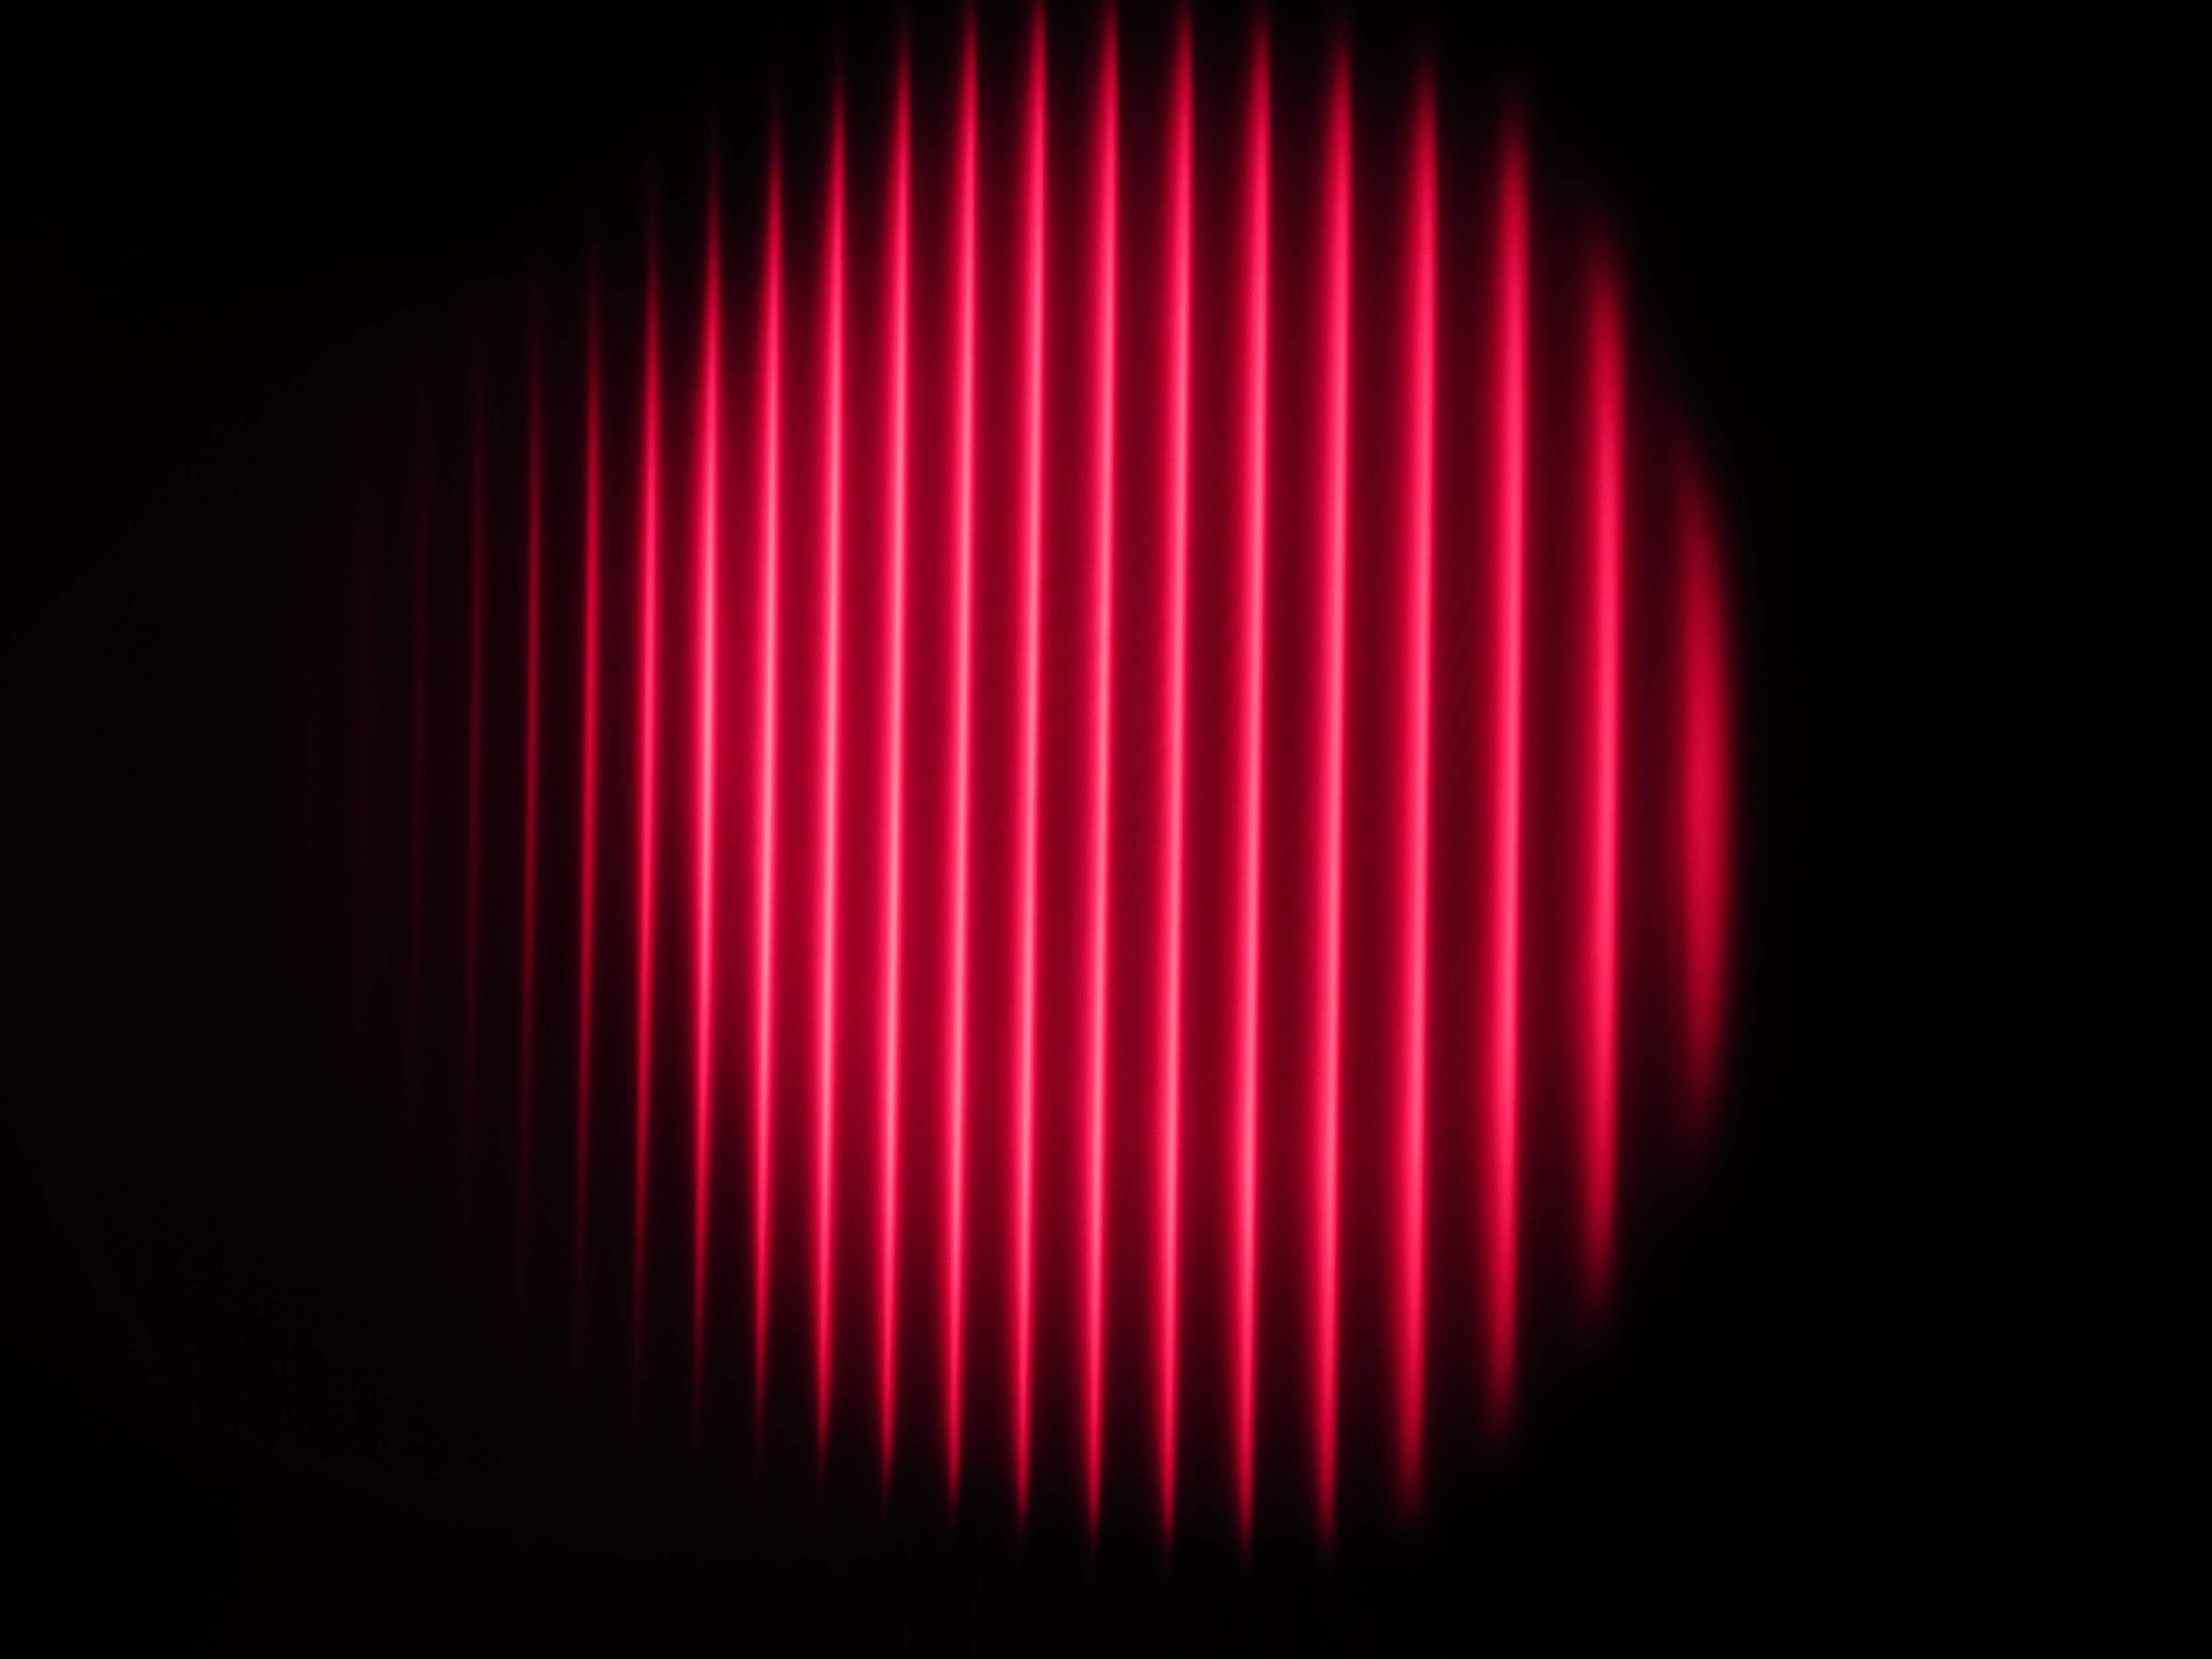
\includegraphics[width=0.45\textwidth,keepaspectratio]{../Bilder/95.pdf}}
    \vspace{0.1\textwidth}
    \subfloat[][]{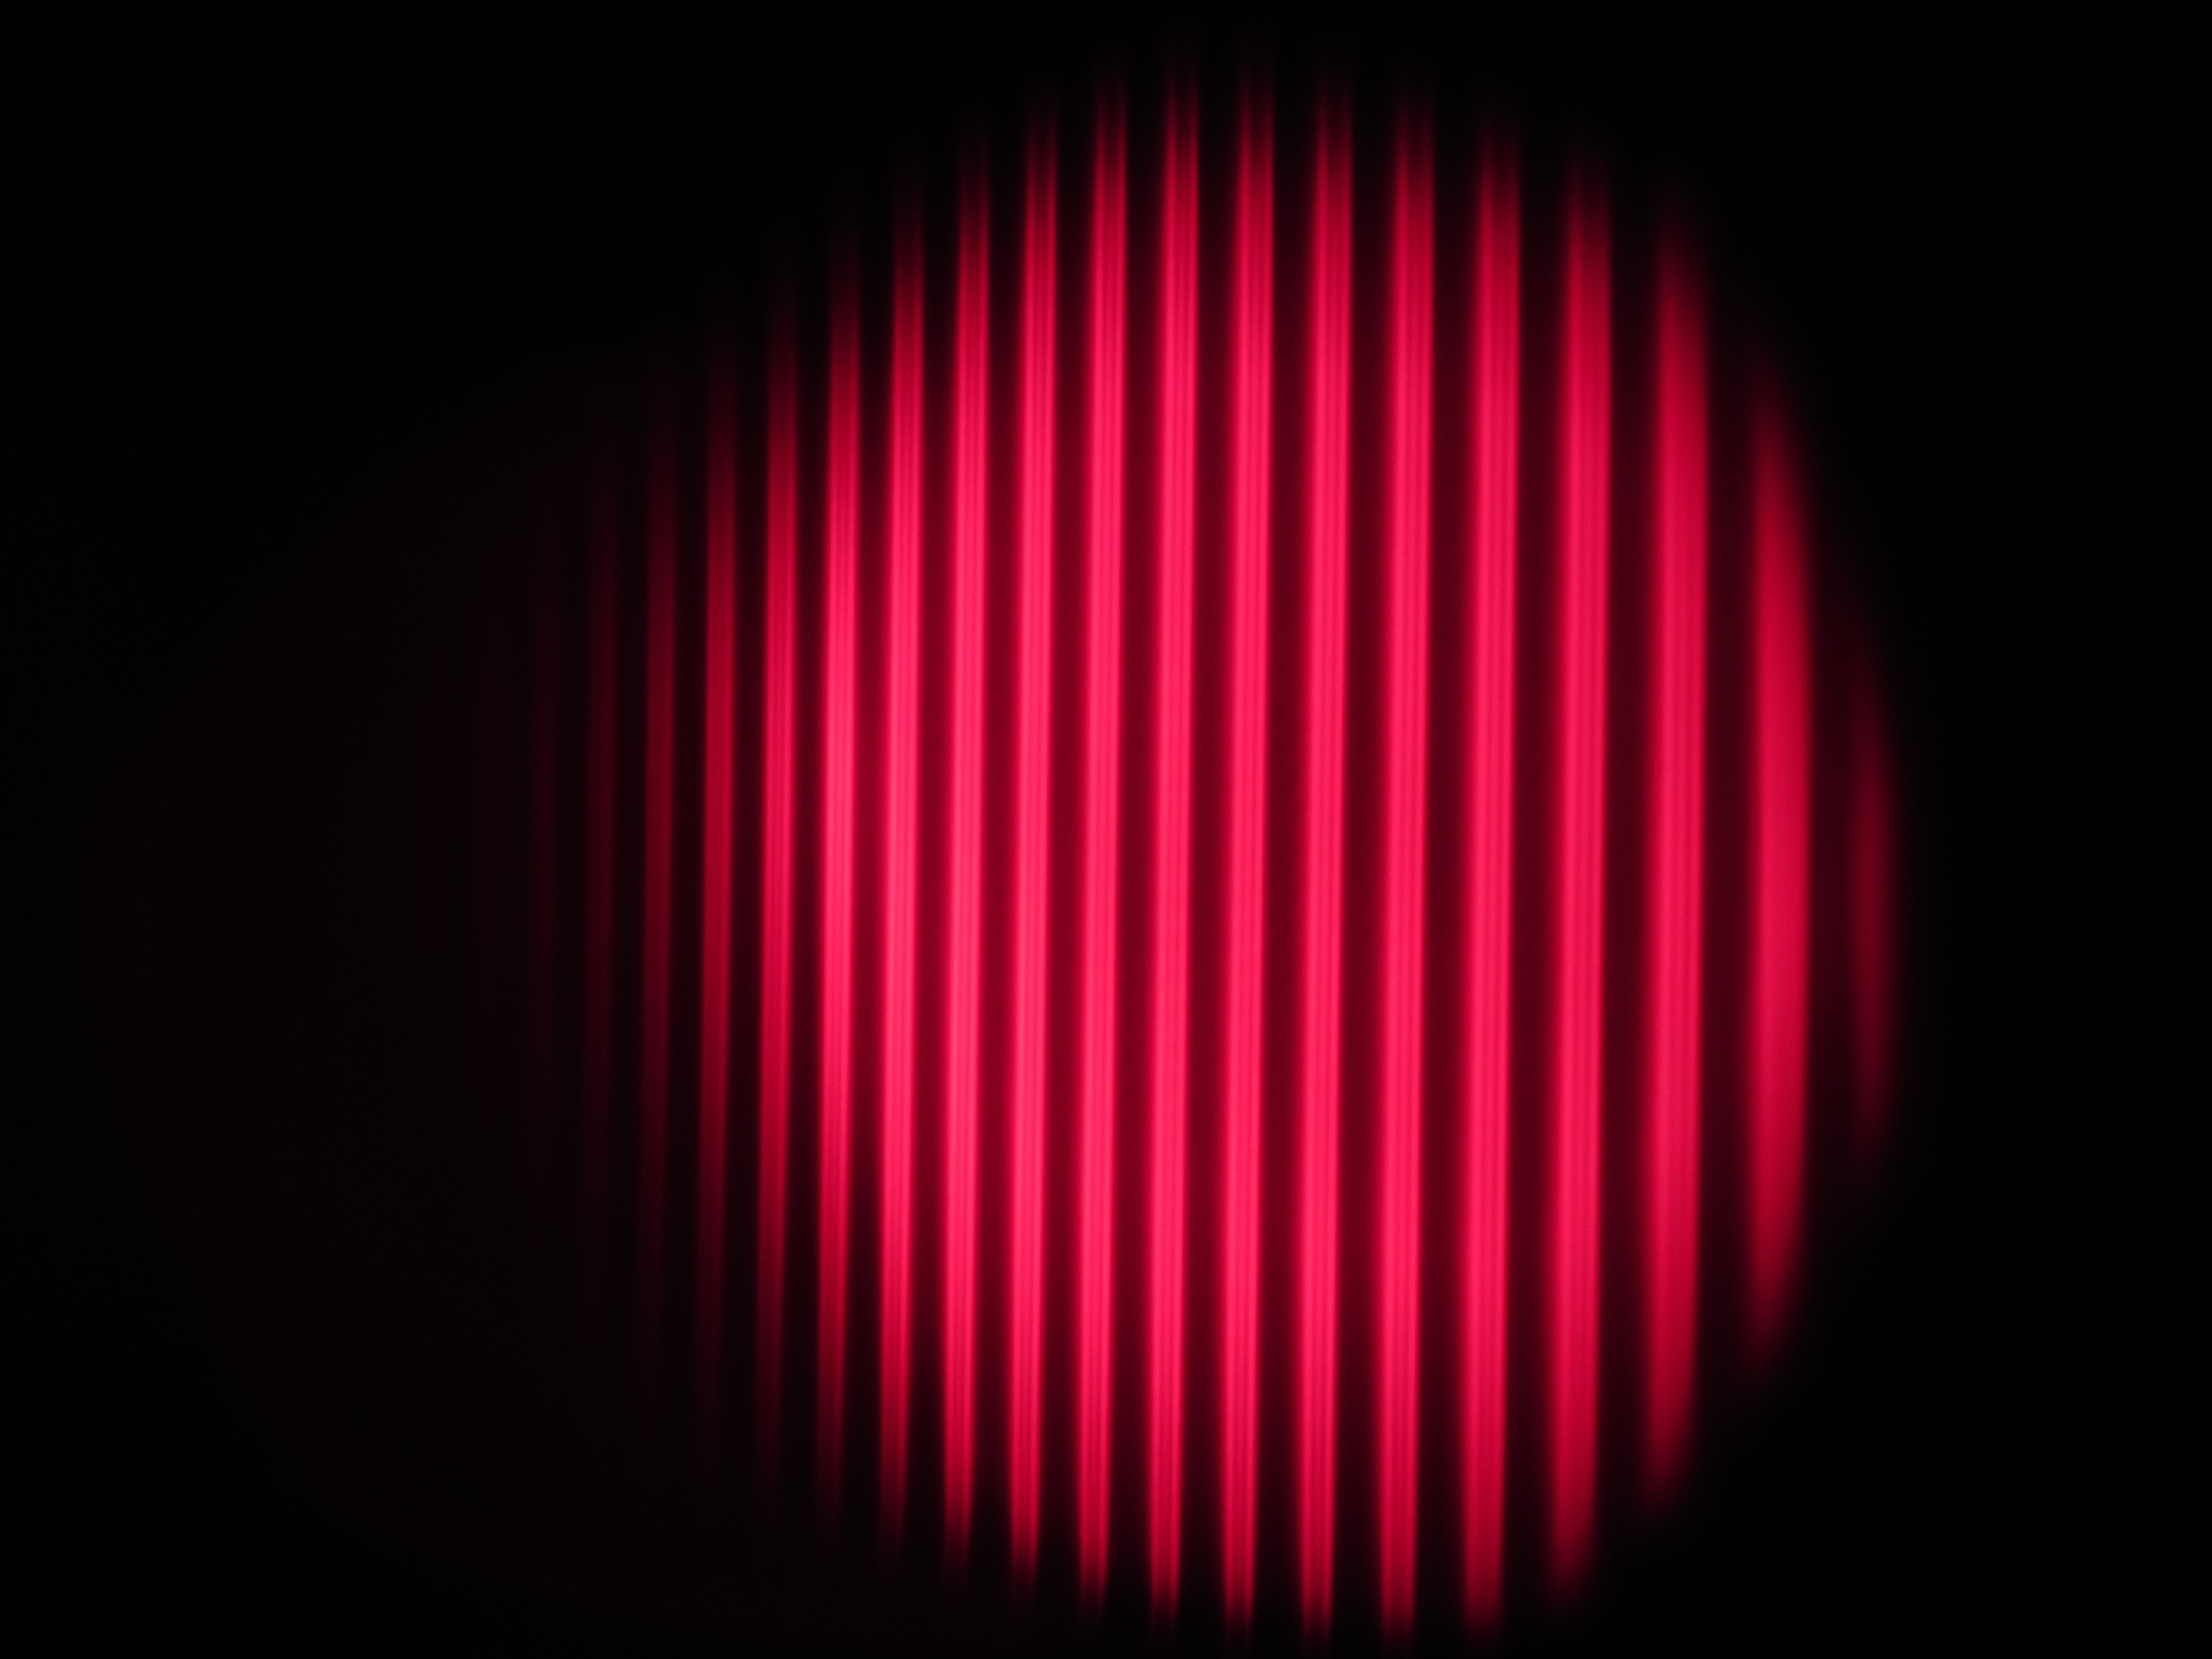
\includegraphics[width=0.45\textwidth,keepaspectratio]{../Bilder/97.pdf}}
    \caption{Messung der roten Spektrallinie für die Bestimmung der Verschiebung $\delta \lambda$ des $\sigma$-Übergangs, (a) ohne Magnetfeld, (b) mit Magnetfeld der Stärke $\SI{394(9)}{\milli\tesla}$.}
    \label{fig:rot_ohne_B}
\end{figure}
\FloatBarrier
Die Verschiebungen können mit der Formel 
\begin{equation}
    \label{eq:Verschiebung}
    \delta \lambda = \frac{1}{2}\frac{\delta S}{\Delta S}\Delta \lambda_{\text{D}} 
\end{equation}
bestimmt werden.
Die Verschiebungen und die benötigten Messwerte sind in Tabelle \ref{tab:rot_Verschiebung} aufgelistet.
\FloatBarrier
\begin{table}
    \centering
    \caption{Messwerte für die Bestimmung der Verschiebung $\delta \lambda$ der roten Spektrallinie und die $\delta\lambda$ Werte. Hierbei werden die $\Delta S$ und $\delta S$ Werte in Pixeln angegeben.}
    \label{tab:rot_Verschiebung}
    \begin{tabular}{c c c}
        \toprule
        $\Delta S$&$\delta S$&Verschiebung $\delta \lambda$ / $\SI{}{\pico\meter}$\\
        \midrule 
        $\num{56.34}$&$\num{23.37}$ &$\num{10.14}$\\
        $\num{56.93}$&$\num{23.98}$ &$\num{10.3}$\\
        $\num{57.53}$&$\num{24.00}$ &$\num{10.2}$\\
        $\num{58.73}$&$\num{26.39}$ &$\num{10.99}$\\
        $\num{59.34}$&$\num{26.37}$ &$\num{10.87}$\\
        $\num{63.52}$&$\num{29.97}$ &$\num{11.54}$\\
        $\num{65.92}$&$\num{28.16}$ &$\num{10.44}$\\
        $\num{63.52}$&$\num{30.56}$ &$\num{11.76}$\\
        $\num{70.71}$&$\num{28.16}$ &$\num{9.74}$\\
        $\num{71.91}$&$\num{28.76}$ &$\num{9.78}$\\
        $\num{76.14}$&$\num{31.17}$ &$\num{10.01}$\\
        $\num{79.70}$&$\num{37.76}$ &$\num{11.58}$\\
        $\num{80.30}$&$\num{35.96}$ &$\num{10.95}$\\
        $\num{90.49}$&$\num{40.15}$ &$\num{10.85}$\\
        $\num{95.89}$&$\num{34.76}$ &$\num{8.86}$\\
        $\num{100.67}$&$\num{44.98}$&$\num{10.92}$\\
        \bottomrule
    \end{tabular}
\end{table}
\FloatBarrier
Aus den $\delta\lambda$ Werten aus der Tabelle \ref{tab:rot_Verschiebung} kann der Mittelwert
\begin{equation*}
    \overline{\delta\lambda} = \SI{10.6(7)}{\pico\meter}
\end{equation*}
für den $\sigma$-Übergang berechnet werden.
\subsection{Aufspaltung der blauen Spektrallinie}
Auch die Aufspaltung der blauen Spektrallinie wird wie im vorherigen Kapitel vermessen.
Hierbei kann allerdings ein $\sigma$ und ein $\pi$ Übergang gemessen werden.
Die Abbildungen für die Bestimmung des $\sigma$-Übergangs sind in Abbildung \ref{fig:blau_sigma} zu sehen.
\FloatBarrier
\begin{figure}
    \centering
    \subfloat[][]{
\includegraphics[width=0.45\textwidth,keepaspectratio]{../Bilder/105.pdf}}
    \vspace{0.1\textwidth}
    \subfloat[][]{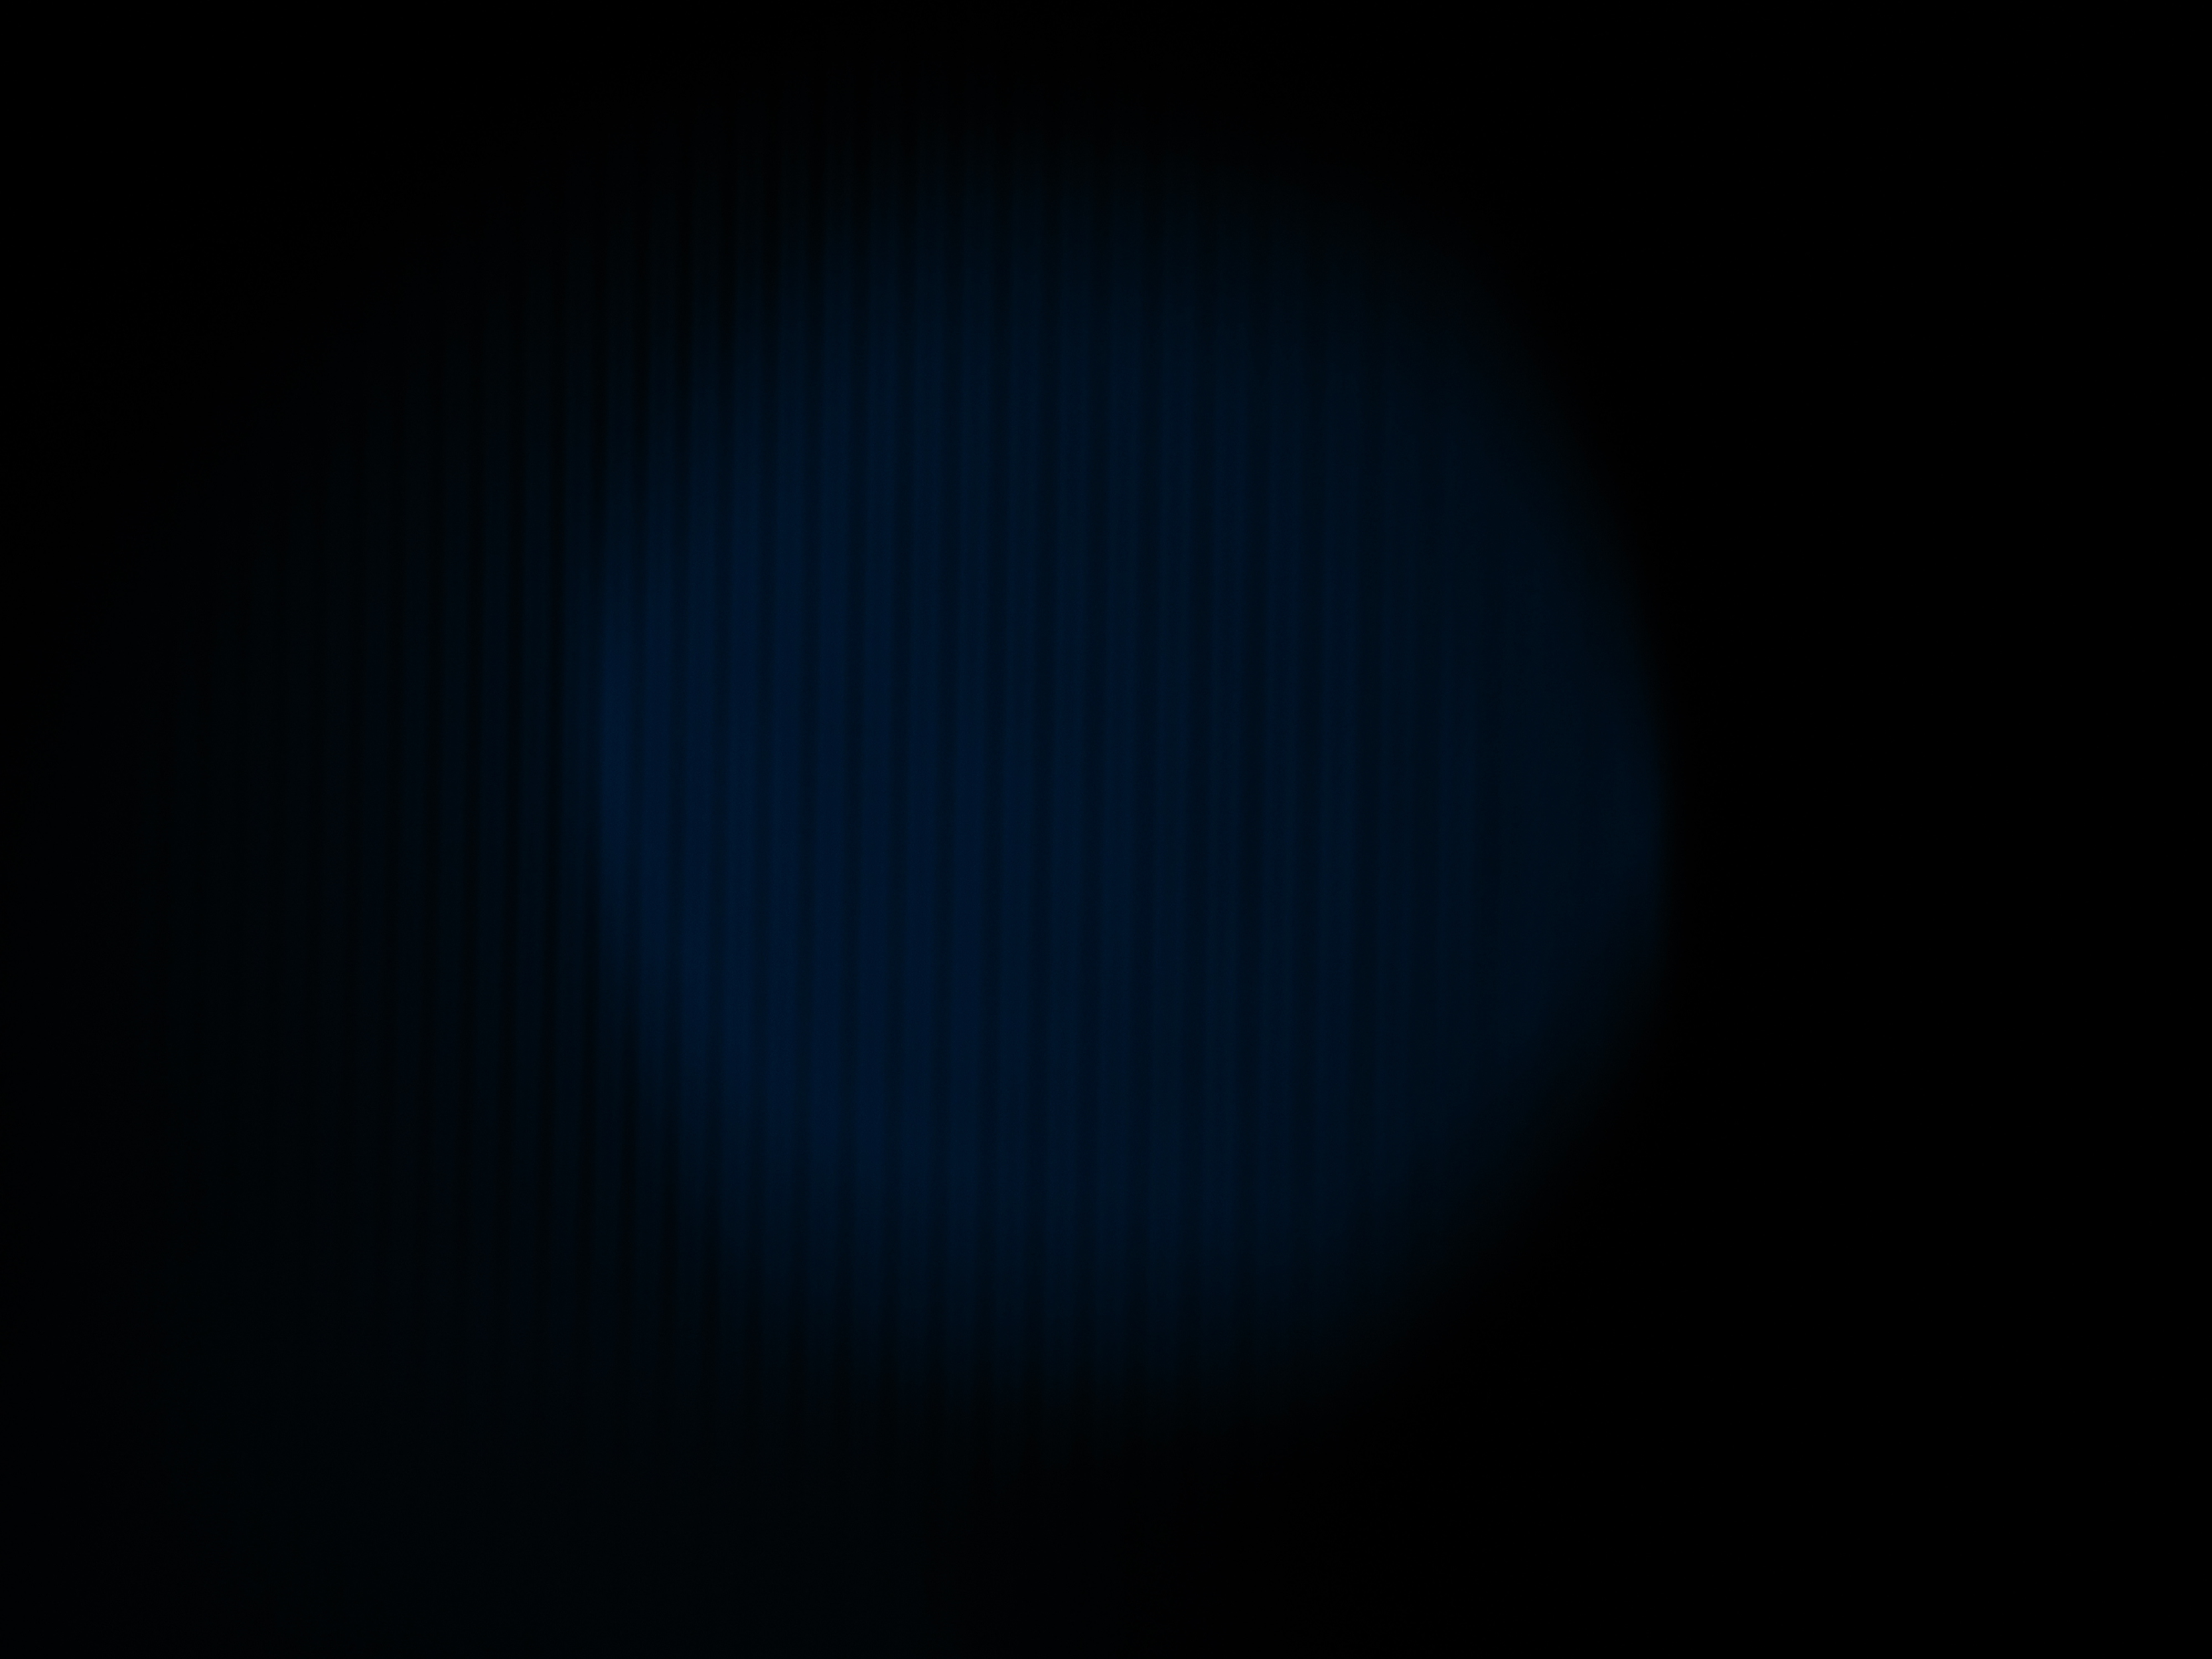
\includegraphics[width=0.45\textwidth,keepaspectratio]{../Bilder/107.pdf}}
    \caption{Messung der blauen Spektrallinie für die Bestimmung der Verschiebung $\delta \lambda$ des $\sigma$-Übergangs, (a) ohne Magnetfeld, (b) mit Magnetfeld der Stärke $\SI{313(8)}{\milli\tesla}$.}
    \label{fig:blau_sigma}
\end{figure}
\FloatBarrier
Die Messwerte sind in Tabelle \ref{tab:blau_sigma} aufgelistet. Mit der Gleichung \eqref{eq:Verschiebung} kann wieder
die Verschiebung der Wellenlänge bestimmt werden.
%\FloatBarrier
\begin{table}
    \centering
    \caption{Messwerte für die Bestimmung der Verschiebung $\delta \lambda$ der blauen Spektrallinie und die $\delta\lambda$ Werte des $\sigma$-Übergangs. Hierbei werden die $\Delta S$ und $\delta S$ Werte in Pixeln angegeben.}
    \label{tab:blau_sigma}
    \begin{tabular}{c c c}
        \toprule
        $\Delta S$&$\delta S$&Verschiebung $\delta \lambda$ / $\SI{}{\pico\meter}$\\
        \midrule 
        $\num{42.39}$&$\num{17.08}$&$\num{5.44}$\\
        $\num{39.83}$&$\num{17.98}$&$\num{6.09}$\\
        $\num{41.10}$&$\num{15.88}$&$\num{5.22}$\\
        $\num{43.65}$&$\num{17.39}$&$\num{5.38}$\\
        $\num{45.34}$&$\num{18.28}$&$\num{5.44}$\\
        $\num{43.65}$&$\num{16.48}$&$\num{5.1}$\\
        $\num{44.50}$&$\num{19.48}$&$\num{5.91}$\\
        $\num{46.19}$&$\num{20.47}$&$\num{5.98}$\\
        $\num{51.27}$&$\num{20.08}$&$\num{5.29}$\\
        $\num{45.76}$&$\num{21.87}$&$\num{6.45}$\\
        $\num{52.54}$&$\num{22.47}$&$\num{5.77}$\\
        $\num{51.70}$&$\num{19.48}$&$\num{5.09}$\\
        $\num{54.24}$&$\num{24.29}$&$\num{6.05}$\\
        $\num{55.93}$&$\num{24.27}$&$\num{5.86}$\\
        $\num{51.69}$&$\num{24.87}$&$\num{6.5}$\\
        $\num{63.56}$&$\num{28.22}$&$\num{5.99}$\\
        \bottomrule
    \end{tabular} 
\end{table}
\FloatBarrier
Die gemittelten $\delta \lambda$ Werte aus der Tabelle \ref{tab:blau_sigma} ergeben 
\begin{equation*}
    \overline{\delta\lambda} = \SI{5.7(4)}{\pico\meter}
\end{equation*}
für den $\sigma$-Übergang der blauen Spektrallinie.
Die Abbildungen für den $\pi$-Übergang sind in Abbildung \ref{fig:blau_pi} zu sehen.
\FloatBarrier
\begin{figure}
    \centering
    \subfloat[][]{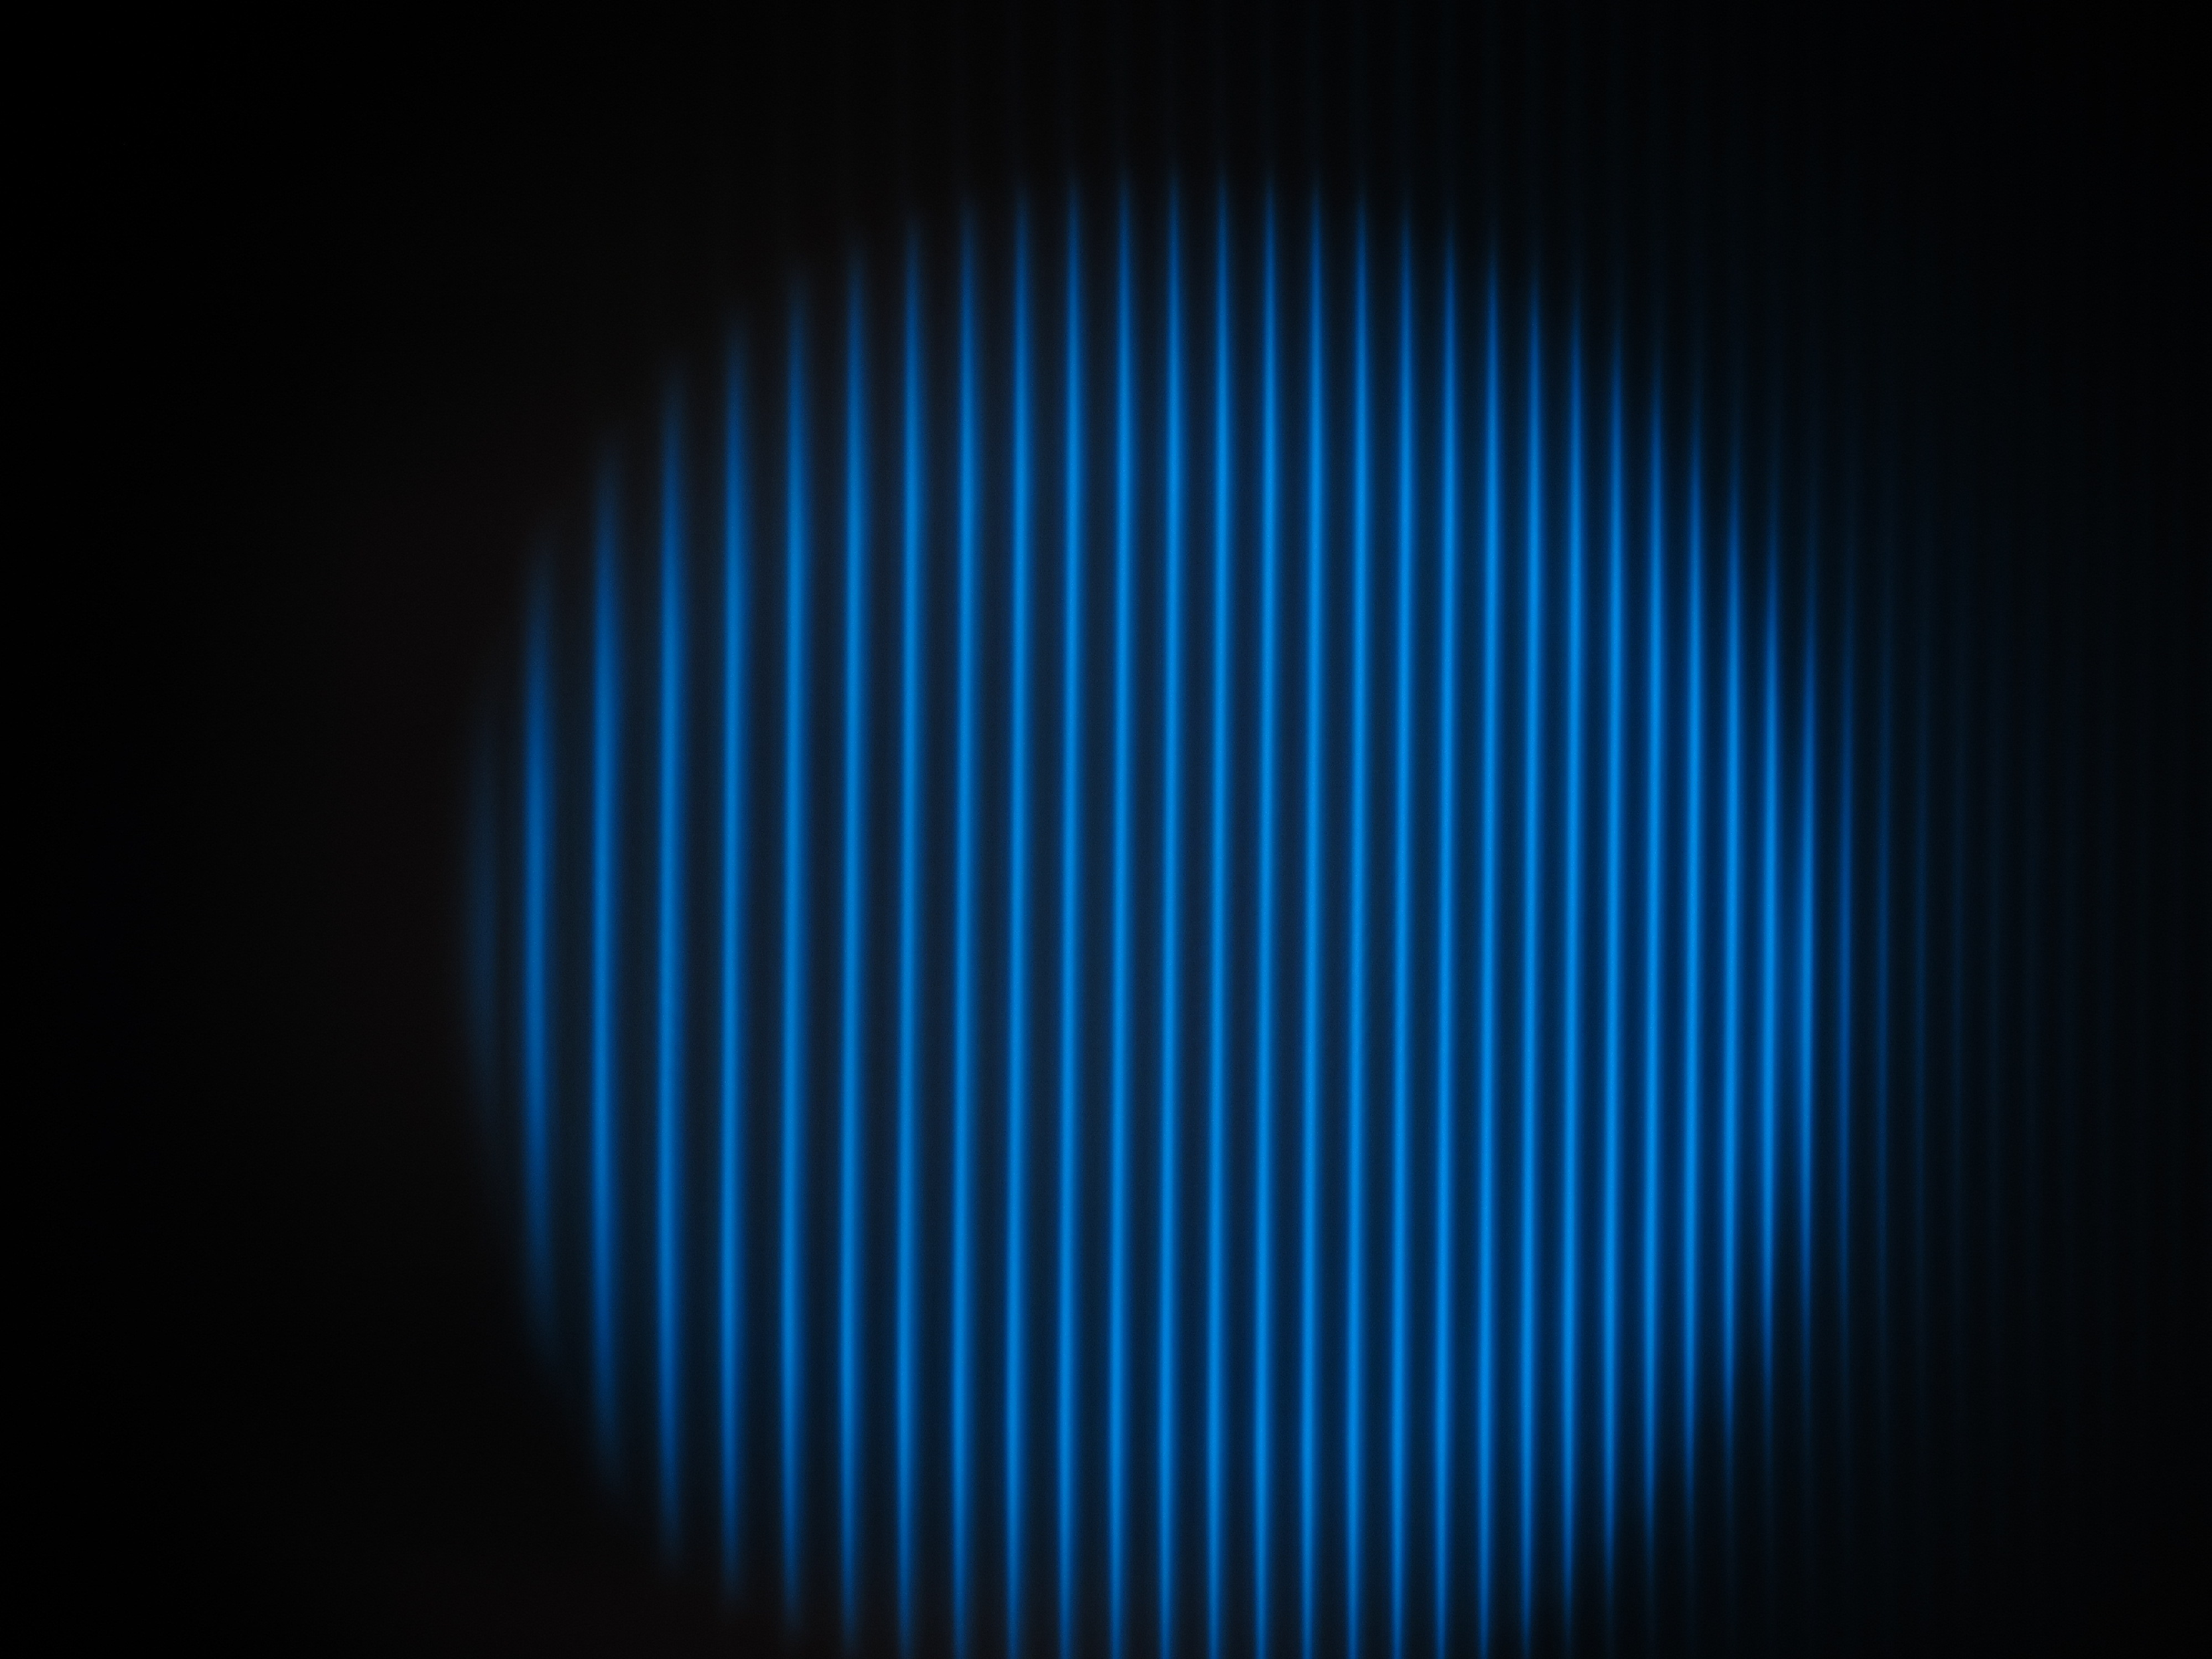
\includegraphics[width=0.45\textwidth,keepaspectratio]{../Bilder/blau_B0.pdf}}
    \vspace{0.1\textwidth}
    \subfloat[][]{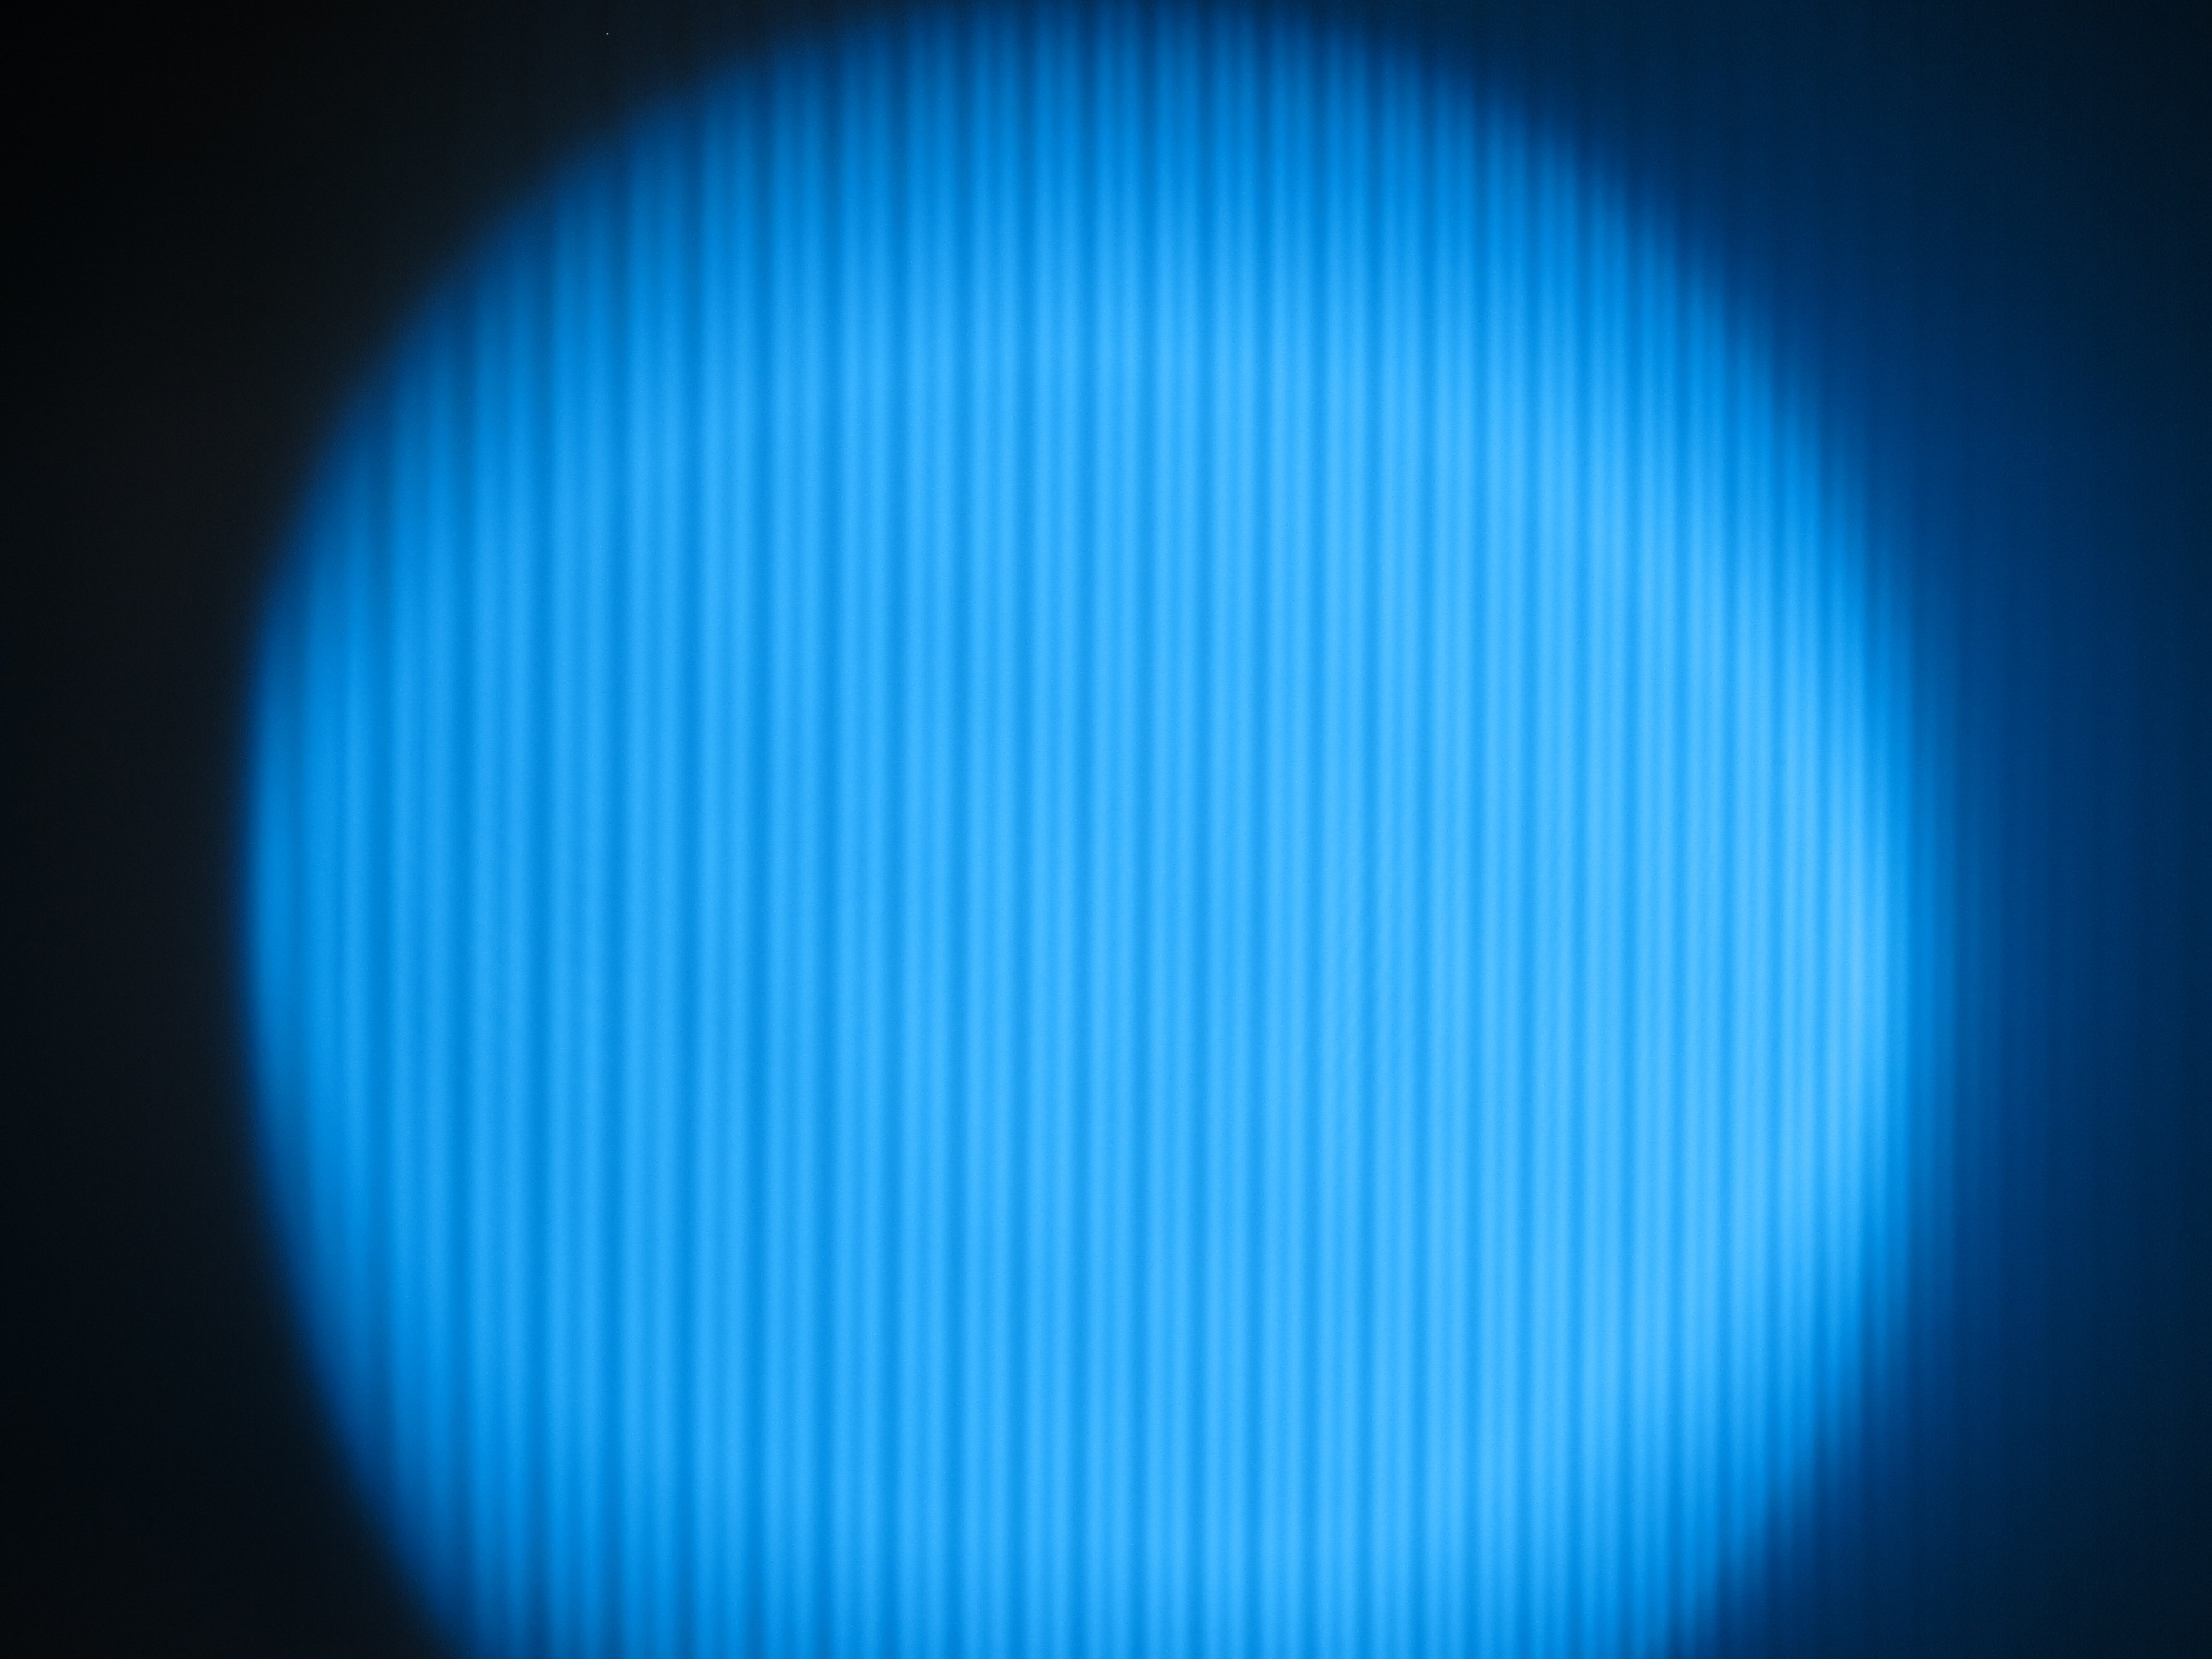
\includegraphics[width=0.45\textwidth,keepaspectratio]{../Bilder/blau_B1009_pi.pdf}}
    \caption{Messung der blauen Spektrallinie für die Bestimmung der Verschiebung $\delta \lambda$ des $\pi$-Übergangs, (a) ohne Magnetfeld, (b) mit Magnetfeld der Stärke $\SI{1009}{\milli\tesla}$.}
    \label{fig:blau_pi}
\end{figure}
\FloatBarrier
Die Messwerte für die Bestimmung der Wellenlängenverschiebung des $\pi$-Übergangs der blauen Spektrallinie sind in 
Tabelle \ref{tab:blau_pi} aufgelistet.
\FloatBarrier
\begin{table}
    \centering
    \caption{Messwerte für die Bestimmung der Verschiebung $\delta \lambda$ der blauen Spektrallinie und die $\delta\lambda$ Werte des $\pi$-Übergangs. Hierbei werden die $\Delta S$ und $\delta S$ Werte in Pixeln angegeben.}
    \label{tab:blau_pi}
    \begin{tabular}{c c c}
        \toprule
        $\Delta S$&$\delta S$&Verschiebung $\delta \lambda$ / $\SI{}{\pico\meter}$\\
        \midrule 
        $\num{66.10}$&$\num{27.97}$&$\num{5.71}$\\
        $\num{58.48}$&$\num{36.87}$&$\num{8.51}$\\
        $\num{63.58}$&$\num{34.32}$&$\num{7.29}$\\
        $\num{60.17}$&$\num{35.18}$&$\num{7.89}$\\
        $\num{57.63}$&$\num{30.94}$&$\num{7.25}$\\
        $\num{53.40}$&$\num{29.66}$&$\num{7.5}$\\
        $\num{52.54}$&$\num{28.81}$&$\num{7.4}$\\
        $\num{51.70}$&$\num{31.78}$&$\num{8.3}$\\
        $\num{50.86}$&$\num{30.51}$&$\num{8.1}$\\
        $\num{49.15}$&$\num{27.12}$&$\num{7.45}$\\
        $\num{47.88}$&$\num{27.15}$&$\num{7.66}$\\
        $\num{45.35}$&$\num{25.85}$&$\num{7.7}$\\
        $\num{47.47}$&$\num{29.24}$&$\num{8.32}$\\
        $\num{44.93}$&$\num{26.69}$&$\num{8.02}$\\
        $\num{44.07}$&$\num{24.58}$&$\num{7.53}$\\
        $\num{43.23}$&$\num{23.31}$&$\num{7.28}$\\
        $\num{41.10}$&$\num{24.58}$&$\num{8.07}$\\
        $\num{42.80}$&$\num{21.19}$&$\num{6.68}$\\
        $\num{38.99}$&$\num{25.46}$&$\num{8.82}$\\
        $\num{41.53}$&$\num{23.73}$&$\num{7.71}$\\
        $\num{39.41}$&$\num{24.15}$&$\num{8.27}$\\
        $\num{37.71}$&$\num{24.16}$&$\num{8.65}$\\
        $\num{39.83}$&$\num{23.73}$&$\num{8.04}$\\
        $\num{36.44}$&$\num{21.19}$&$\num{7.85}$\\
        $\num{37.71}$&$\num{19.92}$&$\num{7.13}$\\
        $\num{37.71}$&$\num{22.46}$&$\num{8.04}$\\
        $\num{34.75}$&$\num{22.46}$&$\num{8.73}$\\
        \bottomrule
    \end{tabular} 
\end{table}
\FloatBarrier
Die gemittelten $\delta \lambda$ Werte aus der Tabelle \ref{tab:blau_pi} ergeben 
\begin{equation*}
    \overline{\delta\lambda} = \SI{7.8(7)}{\pico\meter}
\end{equation*}
für den $\pi$-Übergang der blauen Spektrallinie.
\subsection{Bestimmung des Landéfaktors}
Die Änderung der Energie $\Delta E$ lässt sich durch die Gleichung 
\begin{equation}
    \label{eq:Delta_E_theo}
    \Delta E = \Delta mg\mu_{\text{B}}B
\end{equation}
beschreiben. 
Diese kann auch als Ableitung der Gleichung
\begin{equation*}
    E = \frac{hc}{\lambda}
\end{equation*}
angegeben werden. 
Die Ableitung ist 
\begin{equation*}
    \frac{\partial E}{\partial \lambda}=-\frac{hc}{\lambda^2}.
\end{equation*}
Daraus folgt die Gleichung 
\begin{equation}
    \label{eq:Delta_E}
    \Delta E =\frac{\partial E}{\partial \lambda}\cdot \delta\lambda.
\end{equation}
Die Gleichung \eqref{eq:Delta_E_theo} wird mit Gleichung \eqref{eq:Delta_E} gleichgesetzt und in die Gleichung \eqref{eq:Landeübergang} eingesetzt, um diese nach $g_{\text{ij}}$ umzustellen. Da es sich um 
Energiedifferenzen handelt, wird das negative Vorzeichen vernachlässigt.
Daraus folgt
\begin{equation}
    \label{eq:g_Bestimmung}
    g_{\text{ij}}=\frac{hc}{\lambda^2}\frac{\delta \lambda}{\mu_{\text{B}B}}.
\end{equation}
Die damit bestimmten Landé-Faktoren sind in Tabelle \ref{tab:exp_lande} aufgelistet.
\FloatBarrier
\begin{table}
    \centering
    \caption{Daten für die Bestimmung der Landé-Faktoren und die bestimmten Landé-Faktoren.}
    \label{tab:exp_lande}
    \begin{tabular}{c c c c c}
        \toprule
        $\lambda$ / $\SI{}{\nano\meter}$&Übergang&$B$ / $\SI{}{\milli\tesla}$&$\delta \lambda$ / $\SI{}{\pico\meter}$&Landé-Faktoren\\
        \midrule
        rot $\num{643.8}$ &$\sigma$ &$\num{394(9)}$ &$\num{10.6(7)}$  &$\num{1.39(10)}$\\
        blau $\num{480.0}$&$\sigma$ &$\num{313(8)}$ &$\num{5.7(4)}$ &$\num{1.70(14)}$\\
        blau $\num{480.0}$&$\pi$    &$\num{1009}$   &$\num{7.8(7)}$  &$\num{0.72(6)}$\\
        \bottomrule
    \end{tabular}
\end{table}